\documentclass{article}

\usepackage{graphicx} % for images
\usepackage{amsmath} % for math
\usepackage{amssymb} % for \mathbb
\usepackage{siunitx} % for \SI, \num
\usepackage{hyperref} % for \url{}

% This stuff is for figures
\usepackage{float}
\DeclareGraphicsExtensions{.pdf, .png, .jpg}

% coloring of links for PDF format
\hypersetup{
    colorlinks=true,
    urlcolor=blue,
    linkcolor=black
}

% \c command redefinition (for monospaced font)
\renewcommand{\c}[1]{\texttt{#1}}
% \today command re-definition
%https://tex.stackexchange.com/questions/112932/today-month-as-text
\renewcommand{\today}{\ifnum\number\day<10 0\fi \number\day \space%
\ifcase \month \or January\or February\or March\or April\or May%
\or June\or July\or August\or September\or October\or November\or December\fi\space%
\number \year} 

\begin{document}

\noindent
Rodrigo Becerril Ferreyra\\
CECS 440 Section 02\\
Lab 1\\
\today

%\addcontentsline{toc}{section}{Problem 1.1}
\section{Test Program}
Figure \ref{screenshot:test-program} shows the screenshot of
\c{test-program.asm} running on QtSPIM.

\begin{figure}[H]
    \centering
    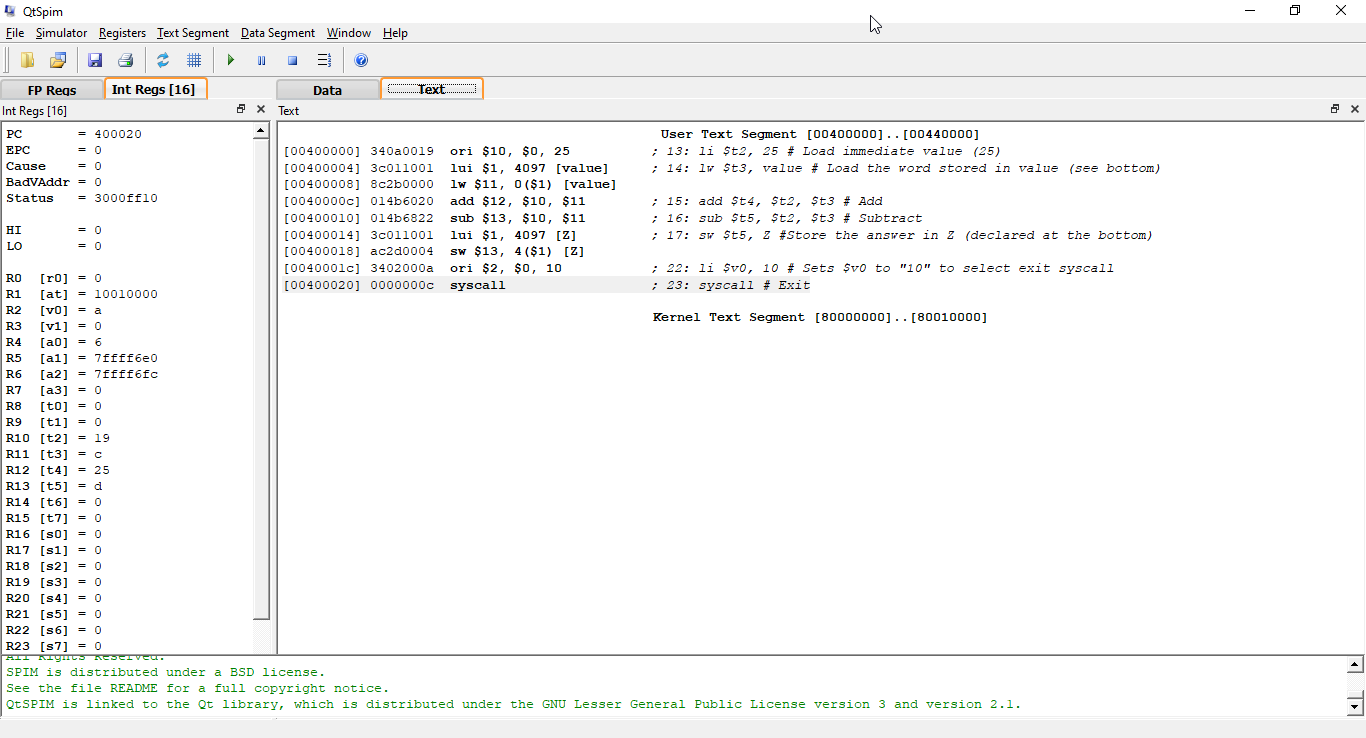
\includegraphics[width=\textwidth]{Images/QtSPIMtestprogram}
    \caption{\c{test-program.asm} (feel free to zoom in).}
    \label{screenshot:test-program}
\end{figure}

\begin{itemize}
    \item Nine total instructions are executed.
    \item The registers \c{\$t2}, \c{\$t3}, \c{\$t4}, and
    \c{\$t5} are all directly used in calculations, along with
    \c{\$v0}, which is used for the \c{syscall}.
    Registers \c{\$at},
    \c{\$a0}, \c{\$a1}, and \c{\$a2} as well as \c{\$sp} are
    all used by the simulated computer automatically, without
    an explicit command.
    \item The address \c{0x10010004} is changed when the command
    \c{sw} is used. This is the address of \c{Z}. (Address
    \c{0x10010000} is also used, but is not changed.)
    It is interesting to note that loading in the address of
    a bit in memory is done in two instructions rather than one,
    because load commands have a limitation of only being able
    to store 16 bits in its last field.
    \item The only \c{syscall} that is used is 10, which
    simply ends the program. If it were not there, QtSPIM
    would give an error when the program tries to go past
    the last instruction.
\end{itemize}

\section{Hello World}
\begin{figure}[H]
    \centering
    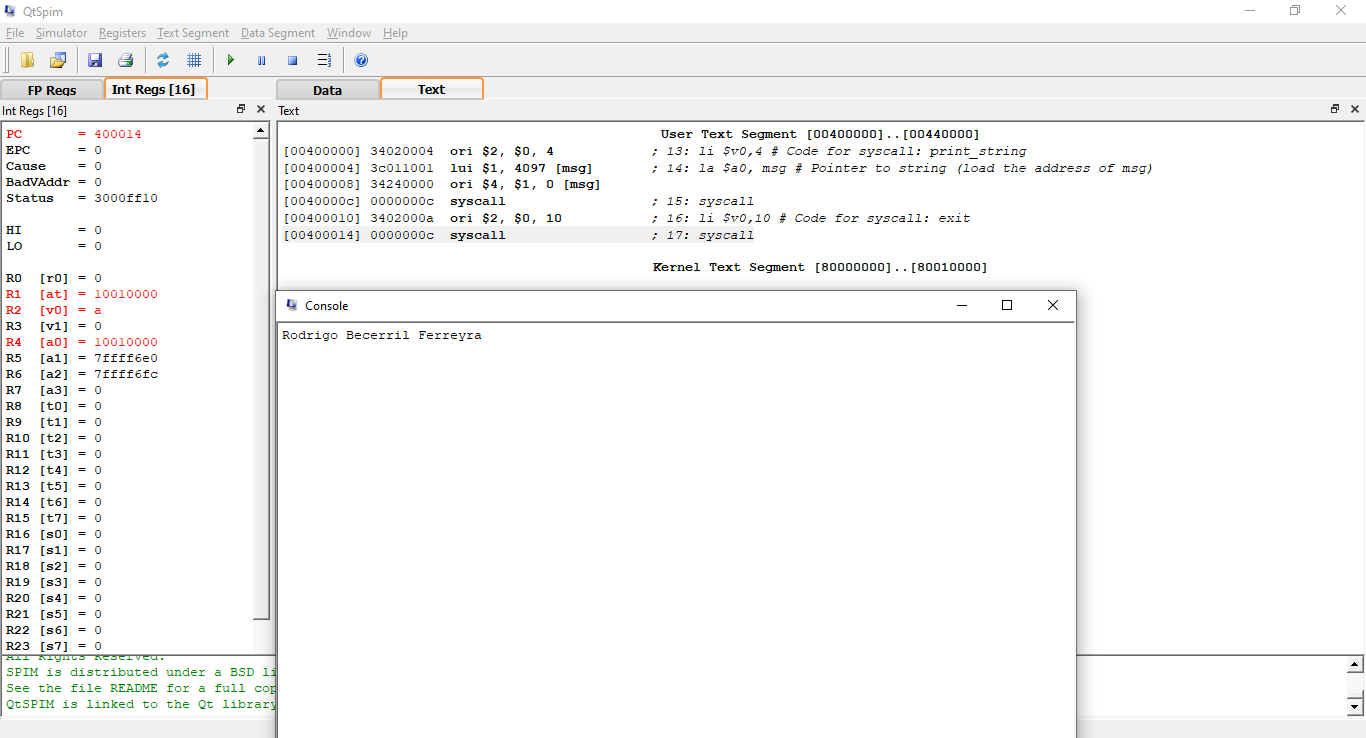
\includegraphics[width=\textwidth]{Images/helloworld}
    \caption{\c{hello-world.asm}}
    \label{screenshot:hello-world}
\end{figure}

\section{Simple Add}
\begin{figure}[H]
    \centering
    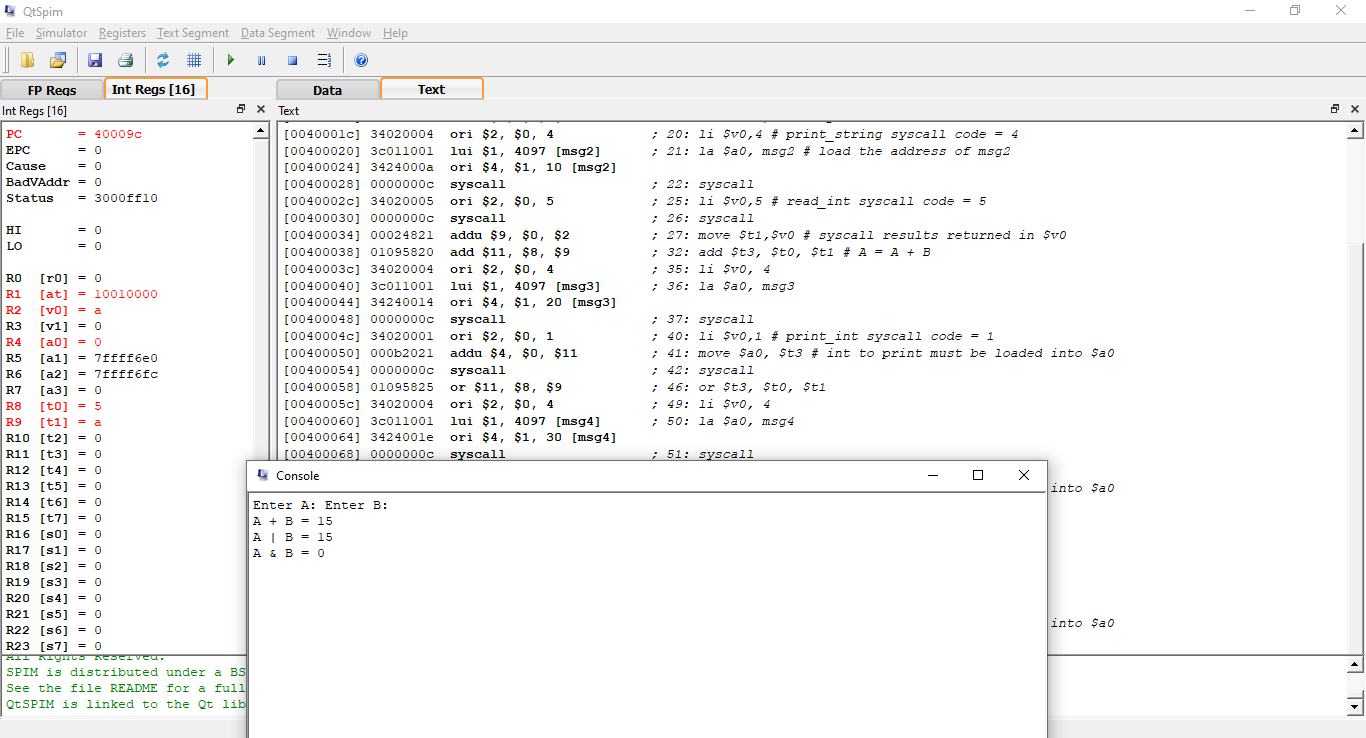
\includegraphics[width=\textwidth]{Images/simpleadd}
    \caption{\c{simple-add.asm}}
    \label{screenshot:simple-add}
\end{figure}

\end{document}
